\documentclass[12pt,a4paper]{article}
\usepackage[utf8]{inputenc}
\usepackage[spanish]{babel}
\usepackage{amsmath}
\usepackage{amsfonts}
\usepackage{amssymb}
\usepackage{makeidx}
\usepackage{graphicx}
\usepackage{lmodern}
\usepackage{kpfonts}
\usepackage{fourier}
\usepackage[left=2cm,right=2cm,top=2cm,bottom=2cm]{geometry}
\author{Rodriguez Lopez Francisco Javier}
\begin{document}

\begin{center}
\LARGE \textbf{Universidad Politecnica de la Zona Metropoilitana de Guadalajara\\}



\includegraphics[scale=1]{Upzmg8.png}  

\large \textbf{Diagrama electrico de la interfaz de potencia}\\
\vspace{2cm}
\large \textbf{Nombre:\\
Guzmán Vázquez Jaime Alan Yamil.\\
Rodríguez López Francisco Javier.\\
\vspace{0.5cm} Matricula:\\
18311861.\\
18311804.\\
\vspace{0.5cm} Carrera: Ingenieria en Mecatronica.\\
\vspace{0.5cm} Materia: Sistemas Electronicos de Interfaz.\\
\vspace{0.5cm} Curso: septiembre-diciembre del 2019.\\
\vspace{0.5cm} Docente: Móran Garabito Carlos Enrique.}


\vspace{3cm}
\small \textbf{10 de Noviembre del 2019}
\end{center}

\section{Introducción:}

Este documento hablara a cerca de la practica que se realizo anteriormente, la practica consiste en generar  con un voltaje de entrada pequeño un incremento de voltaje en la salida del circuito mediante capacitores y push button, esta parte sera mejor explicada en el apartado de desarrollo en donde se hablara a cerca de todas las condicionantes de este tipo de circuito, así como los riesgos que podría traer puesto a su gran inestabilidad y sus beneficios grandes como el incremento grande del voltaje.\\
\\De este reporte resaltaremos dos grandes partes que son el apartado de resultados y el apartado de desarrollo en donde el apartado de desarrollo explicara el como se armo el circuito, las variables que intervinieron en el mismo, como podemos controlar el cambio mismo del incremento de voltaje y su velocidad de descarga así como los factores que lo intervienen.\\
\\
El apartado resultados mostrara las evidencias o variables que fueron salieron del mismo circuito para que el apartado desarrollo tenga coherencia y ser muestren lo que el circuito físico nos demostró, esta sera básicamente la dinámica que se manejara en este reporte de practica para demostrar el circuito realizado. \\

Ademas de los puntos ya mencionados también se hablara acerca de las diferentes aplicaciones de este circuito debido a su peculiaridad y forma de operar así como de sus características y como puede ser implementado en el ámbito profesional o empresarial y como se liga este circuito con el que se estudiara próximamente con la practica numero 9 que esta trata  de disminuir el voltaje en el circuito.


\section{Objetivo:}
Conocer el arreglo, para el paso de corriente alterna a directa, por medio de capacitores, y diodos.\\ 

\section{Materiales:}
\begin{itemize}
\item Capacitores electroliticos (100uF a 63v, 220uF a 50Vv, 10uF a 50V).
\item Diac.
\item Potenciometro de 100k.
\item Puente de diodos (RS206L).
\item Resistencias (2.2k y 100k).
\item Transformador (127vca-16vca).
\item Triac (TYN1225N).
\end{itemize}
\newpage
\section{Procedimiento:}
Para el mejor entendimiento de esta practica, se establece, ñas formas y arreglos que se les puede dar a la transformacion de corriente alterna a continua, siendo está la forma en la que mas comunmete se hace, que es a traves de capacitores, y diodos, para la rectificacion, y el almacenamiento de la carga que va transmitiendo la fuente de poder a la que lo estamos alimentanmdo en este caso, a un to,a corriente directo, para la buena implementacion de esto, el trajsofrmador, se pone, como una fuente de poder, la cual transofrma la energia alterna, y hace que en su transpaso, por su enbobinado, se traspase, a un volatje alterno menor, de criterio este, nos funciona, para un regulador de corriente, asi pues, guiando todo el problema al transformador, y no a nuestro circuito.\\

El diagrama a realizar en esta practica, y evidencia, es en generacion, eso, poder tener el control, en la sujestion, que se tenga que manejar la corriente y el voltaje alterno, y como este nos puede ser de ayuda, a la realizacion de una fuente mas sofisticada, y de mayor arreglo, en terminos de energia alterna. El diagrama utilizado es en cuestion el siguiente:\\

\begin{center}
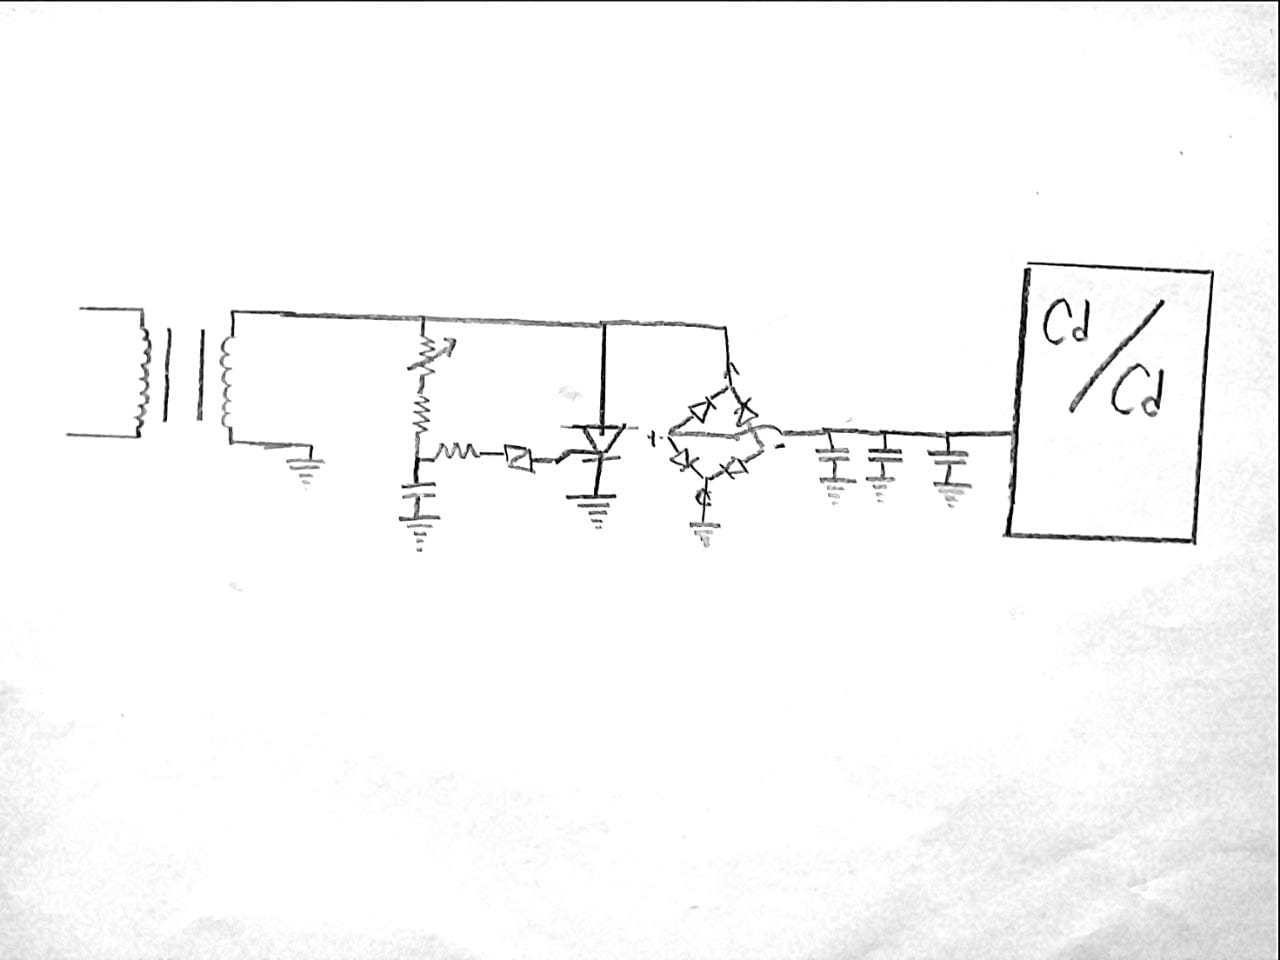
\includegraphics[width=10cm]{esquema.jpeg} 
\end{center}

Como se muestra en el esquematico, esta es el arreglo, que se tiene que tener por etapas, para la conmutacion de la potencia disipada, a partir del voltaje y corriente transmitidos. Esto se tiene por etapas, siendo la etapa 1, la entrada del transformador, esto es lo que hace la conductividad posible, ya que el campo magnetico 	que genera al ser, mayor, retaer el voltaje hasta cierto punto el cual sea manejable. La segunda etapa dirigida por el Triac, este es de suma importancia, que sea de dura potencia, ya que si no lo es, se empezara a calentar, nuestro sistema de control, que en este caso, es para regular el flujo de corriente, y que este no sea excesivo, la etapa 3, constituida, por la entrada del puente rectificador, y los capacitores, esta zona, es la que regula de mejor estancia, la salida de voltaje, potencia y corriente, que lo establece en este punto a directa, y la entrada del Boost, o convertidor de voltaje CD/CD, dobla el voltaje que tenemos a la salida, generando asi, un total de 32v en salida de corriente directa, el cual manejamos, con un Triac (MOC-502R) de menor potencia, que el puesto en primera estancia, ya que a este punto, no se necesita de una potencia grande, por que la conmutacion de corriente alterna, ya a sido covertida y establecida.\\

Teniendo en claro, cada una de las etapas, a manejar, y de ello, a establecer en las pruebas fisicas, nos queda establecido, un sistema de CA a CD, en control absoluto, recalcando, que en la primera estancia, se requiere de componenetes, de alta potencia, ya que la corriente que se arroja, a partir de la conexion directa al enchufe, es de mayor intensidad, y los componentes, de baja potencia, no resistirian.\\

Nota: Se requiere, de un potenciometro, para la mejora de regulacion, a partir de la descarga que sufran los capacitores.

\section{Resultados:}

Establecido, cada una de las etapas, a manera fisica, comprobadas en la protoboard, no queda un sistema de covertidor, alterna directa, a paritr de la rectificacion, y capacitancia, que se tenga, y como esta queda establecida, en este punto, en este caso, siendo un convertidor, de mejor y mayor control, estableciendolo, en una interfaz de potencia, tal y como se ha estado trabajando, a lo largo de este curso, desde baja potencia, hasta potencia alta, los resulatdos generados, son en cuestion, la generacion del brinco de corriente, hasta el doblado de la misma, controlando todo, con el mismo Triac, que se tiene a disposicion misma.\\

El armado de este, genera los resulados ya mencionados, y la resolucion de ellos, a partir de la generacion de potencia que se tenga, y como es que se tenga esta potencia didipada. Quedando en manera fisica de la manera siguiente:

\begin{center}
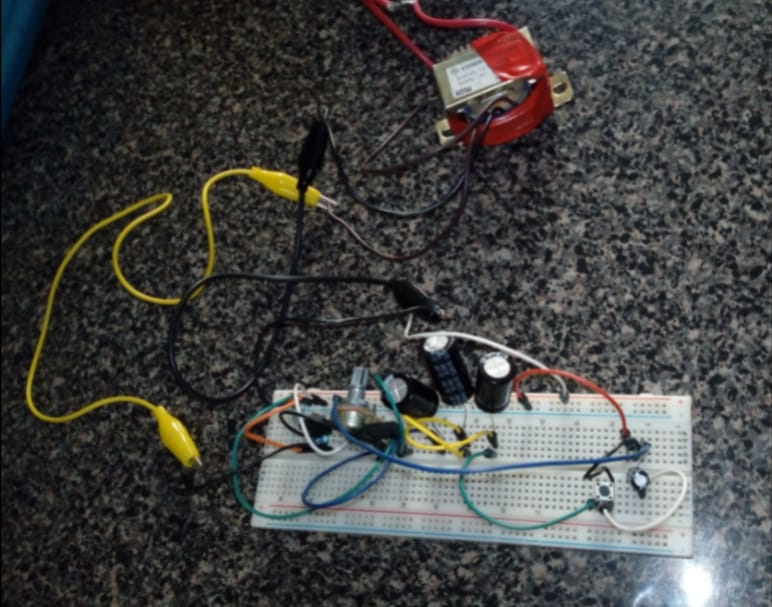
\includegraphics[width=9cm]{Fisico.jpeg} 
\end{center}

La generacion y el acomodo, que se le da a nuestra protoboard, es la generacion de la resultante, la cual es el lanzamiento, del voltaje de corriente directa, como se aprecia el potenciometro, en generacion y control a la potencia que es disipada, en el sistema y como esta es controlada por el Triac que es conectado, en generacion y siendo este conetado no de forma directa al transofmador, sino, pasando por un control, de sistemas conmutados, tales, omo resiswtencias, y un Diac, el cual nos garamtiza el mejor control y sin fallas, de la rectificacion que se tenga en el anodo del Triac, asi como en el gatillo.\\

Las pruebas, para tenerlo mas en cuenta, es la guia de un multimetreo, para ver el voltaje que se genera a partir del paso que hace la corriente, conectando las puntas de prueba, una a la salida de los condensadores, y otra directa a tierra, ya que este punto de las tierras, se sabe que todas son cmunes, y de ello, las conexiones sin riesgo, de quemar, el circuito, ni el multimetro.

\section{Conclusión:}

\textbf{Jaime Guzmán:}\\
Este circuito boost es un circuito que tiene implicaciones muy útiles puesto que mediante el uso de capacitores puede hacer que el voltaje de salida sea mucho mayor al valor de entrada con capacidades dependiendo de el valor del capacitor un incremento de hasta 6 veces mas de lo se tenia de valor de entrada, lamentablemente este circuito es muy inestable por lo que podría se peligroso puesto que este podría tener cambios bruscos de voltaje o incluso poder generar cortos circuitos en el mismo, por este tipo de cuestiones este circuito no es tan seguro pero sin embargo tiene aplicaciones reales en el mundo de la electrónica ya que puede estabilizarse.\\

\textbf{Francisco Ródriguez:}\\
La generacion, y el controlamiento de la potencia que puede ser disipada, a partir de los componentes utilizados, en un sistema de rectificacion y condensacion, es algo que se utiliza de manera eficiente, en sistemas mas complejos, como la prueba de ello, la practica realizada, a partir de la generacion del doblador de voltaje, asi como el paso, por sistemas mas comunes, como potencia de alta estancia, la cual es mas comun utlizar esto, en sistemas, de proyectos mecanicos, el cual tenga que generar a partir de la gran potencia disipada, el movimiento de motores, asi como de sistemas de movimiento en los cuales se necesite, un campo magentico mejor y de mayor corriente.\\
Dado el aprendizaje generado, a partir de estas practicas, y de un sistema de estudios, es lo que nos puede dar guia, a la mejor utilizacion de esto, para la generacion de un proyecto, el cual requiera, de los conocimientos, de potencia, control de ello, y un sistema el cual nos pueda ser de eficiencia, mayor que un simple video de youtube.\\

\textbf{\Large Referencias:}\\

Carlos Enrique Moran Garabito, Sistemas Electronicos de Interfaz, Curso: Sep-Dic 2019 c, Diagramas electricos de interfaz de potencia.

\end{document}